% Ingenieurpraxis
\def\mytitle{realtime FoG detection and hardware implementation}
\def\mykeywords{Freezing of gait, feature extraction, feature selection, gait features, fisher discrimination analysis, DAPHNET}
\def\myauthor{Wei Zhaoxiong}
\def\contact{ge25zir@mytum.de}

\documentclass[article]{article}

\usepackage[a4paper,outer=1.5cm,inner=1.5cm,top=1.75cm,bottom=1.5cm]{geometry}
\twocolumn
\usepackage[utf8]{inputenc}     % Zeichenkodiezrung UTF-8
\usepackage[english]{babel}     % Deutsche Sprache und Silbentrennung
\usepackage{graphicx}           % Bilder
\usepackage[colorlinks,linkcolor={black},citecolor={blue!80!black},urlcolor={blue!80!black}]{hyperref}
\usepackage[parfill]{parskip}   % Stop indentation on new paragraphs
\usepackage{watermark}          % 
\usepackage{lipsum}             % Blindtext
\usepackage{xcolor}             %
\usepackage{listings}           %
\usepackage{float}              %
\usepackage{titlesec}           % 
\usepackage{amsmath}            % Formeln
\usepackage{algorithm2e}        % PseudoCode
\usepackage{caption}
\usepackage{subcaption}
\usepackage{xcolor,colortbl}
\captionsetup[figure]{font=footnotesize}

\renewcommand*\familydefault{\sfdefault}
\graphicspath{{./img/}}
\hypersetup{pdfauthor=\myauthor,pdftitle=\mytitle,pdfkeywords=\mykeywords}

\titlespacing{\subsection}{0pt}{\parskip}{-3pt}
\titlespacing{\subsubsection}{0pt}{\parskip}{-\parskip}
\titlespacing{\paragraph}{0pt}{\parskip}{\parskip}
\newcommand{\figuremacro}[5]{
    \begin{figure}[#1]
        \centering
        \includegraphics[width=#5\columnwidth]{#2}
        \caption[#3]{\textbf{#3}#4}
        \label{fig:#2}
    \end{figure}
}

\lstset{
	escapeinside={/*@}{@*/}, language=C++,
	basicstyle=\fontsize{8.5}{12}\selectfont,
	numbers=left,numbersep=2pt,xleftmargin=2pt,frame=tb,
    columns=fullflexible,showstringspaces=false,tabsize=4,
    keepspaces=true,showtabs=false,showspaces=false,
    backgroundcolor=\color{white}, morekeywords={inline,public,
    class,private,protected,struct},captionpos=t,lineskip=-0.4em,
	aboveskip=10pt, extendedchars=true, breaklines=true,
	prebreak = \raisebox{0ex}[0ex][0ex]{\ensuremath{\hookleftarrow}},
	keywordstyle=\color[rgb]{0,0,1},
	commentstyle=\color[rgb]{0.133,0.545,0.133},
	stringstyle=\color[rgb]{0.627,0.126,0.941}
}



\title{Ingenieurpraxis\\\mytitle}
\author{\myauthor\hspace{1em}\\\contact\\Technische Universität München}
\date{\today}
\sloppy


\begin{document}
\maketitle

% ABSTRACT
\begin{abstract}
    Freezing of gait (FoG) is an abnormal gait pattern that accompany Parkinson's disease(PD). During such short, temporary episodes, the patient is not able to move the feet forward despite the intention of walk. According to  \cite{RAS}, a sequence of rhythmic stimuli is able to help patient to walk again during FoG. Therefore, it is important to detect FoG pattern at the very beginning or even before it comes.
    
    In this paper, we tried to extract and select gait features using DAPHNET dataset. A fisher discrimination analysis and feature thresholding is applied to further reduce its dimension. Besides, we proposed a new evaluation standard that focus on improving the user experience and tune relevant parameters based on it. In the end, the algorithm is implemented in a source-constrained device.
    
\end{abstract}  
\textbf{Keywords -- }{\mykeywords}

% Introduction
\section{Introduction}
    Parkinson's disease (PD) is the second most common aging-associated neurodegenerative disorder \cite{PD}. It is characterized by motor features such as muscular stiffness, resting tremor, hastening of the gait(festination) and poor postural stability. Freezing of gait (FoG) is one of the symptoms of PD, during such sudden and short episode, the patient experiences gait disturbance ranging from complete sudden akinesia to milder leg trembling or short shuffling steps events, usually described by patients as feeling the feet stuck to the floor. These symptoms result in emotional stresses and reduced quality of life \cite{PD1}. However,there is still no effective treatment or drug-resistant against such disease \cite{medicin}.
    
    The work of Hausdorff et al. shows rhythmic auditory stimulation (RAS) was shown to be particularly effective at improving gait among PD patients \cite{RAS1}. In their experiment, regular metronome ticking sounds were applied as RAS with a rate of 110\% compared to the natural walking rate of tested patient.This served to improve gait stability and speed.
 	
 	Since unnecessary ticking sounds during normal walking can be annoying for patient and we want to only provide RAS during an actual or impending FoG event, a realtime detection of FoG is important.
 	
 	  
 	A variety of methods have been proposed to detect FoG. Moore et al. used an Inertial Measurement Unit (IMU) mounted around a shank, and defined a freeze index(FI) using power spectrum analysis of accelerometer signals \cite{FI}. Each patient use individually calibrated thresholds to recognize FoG. The experiment shows that 89\% of FoG event can be detected, However, 10\% of non-FoG events can generate false alarm. 
 	
 	Based on this, Bachlin et al proposed a real-time FoG detection algorithm combines the FI with a second power threshold to discriminate FoG from normal gait, resulting in higher sensitivity (88.6\%) and specificity (92.4\%) \cite{FI1}.
   
    Besides, there are also several machine learning based approaches that exploiting the data set. Florenc et al. applied kernel-lda to the accelerometers' raw data to reduce the dimension of features. Then a k-nearest neighbor algorithm (k-NN) was used to classify gait in pre-FoG, no-FoG and FoG \cite{Flo}. 
    
    Natasa et al. extract several features from raw data and using Boruta algorithm to reduce the dimension, they make a comparison of result using classifiers like Support Vector Machine, Random Forest and k-NN \cite{ML}.
    Similarly, Parisa et al. collected  inertia and physiological signals to extract freezing patterns, the set of features are fed into a Fully-Connected-Neural Network(FCNN) to learn and predict freezing episodes \cite{symptoms}.
    
    Considering that we are using source-constrained wearable devices, some methods can be too expensive to implement, such as parameters of FCNN takes too much memory space and computational resources and it may hard to meet the requirement of real-time. We are not going to consider it as an option in our setup.

 
    
% Approaches tries
\section{Approaches Pursued}

	In this research, I tried several methods mentioned before \cite{FI1} \cite{Flo} \cite{ML}, for some paper I cannot get the desired result because of insufficient understanding of background. In the end, I find a method which yields the best result and I'm going to focus more on talking about it.
	
 	The DAPHNET Freezing of Gait dataset is used for this research \cite{FI1}. This dataset consists of sensor data extracted from individuals with PD. Three tri-axial accelerometers were placed at the shank (just above the ankle), thigh (just above knee) and lower back to collect acceleration in three axes with a sample rate of 64Hz.

	The dataset include data from 10 patients, they are asked to perform walking in straight line, walking with numerous turns and some daily living tasks. The label is done by two physiotherapists using video recording. During the test, two patient did not show any symptoms of FoG, so they are excluded in this research. In total this dataset collected five hundred minutes of data and 237 FoG events happened within this time, half of the FoG episodes lasted less than 5s and most part lasted less than 20s (93.2\%). Therefore, this is an unbalanced dataset that consists much more non-FoG periods than FoG episodes. 


    In the beginning, I tried to implement the approach of Florenc \cite{Flo}. First, all windows preceding FoG windows are labeled as pre-FoG window, this gives us a third class. Then kernel LDA is applied to the raw data to reduce dimension and k-NN is used as a classifier.  However, I failed to separate classes in the test set by using kernel-lda. Also, the author informs that his work does not perform well when it comes to larger data set. So I stopped on working with this algorithms.
    
    Another machine learning algorithm I tried is Neural Network(NN), however, with limited number of weights and layers allowed, it's hard to do the classification correctly.
    
    According to my observation, the reason for the failure of employing  machine learning methods could be the followings. First of all, the data set is not quite balanced, the FoG labeled data is far less than non-FoG data set.  Second, there might be some miss-labeled data. Since the data set is labeled with eye observation, it is possible the detection of FoG is slower than it should have been. Considering that machine learning methods are purely data-driven, such problems with the dataset could have huge impact on the result.

    After a conversation with my advisor, I change the research target to gait cycle analysis. This is a study that is used to assess and treat individuals with conditions affecting their ability to walk. From the data set, it is possible to extract features like walking speed and cadence. The gait analysis construct the basis of new method. The general procedure is shown in figure \ref{fig:procedure}. More detail information can be found in next section.
    
    
    \begin{figure}
    	\centering
    	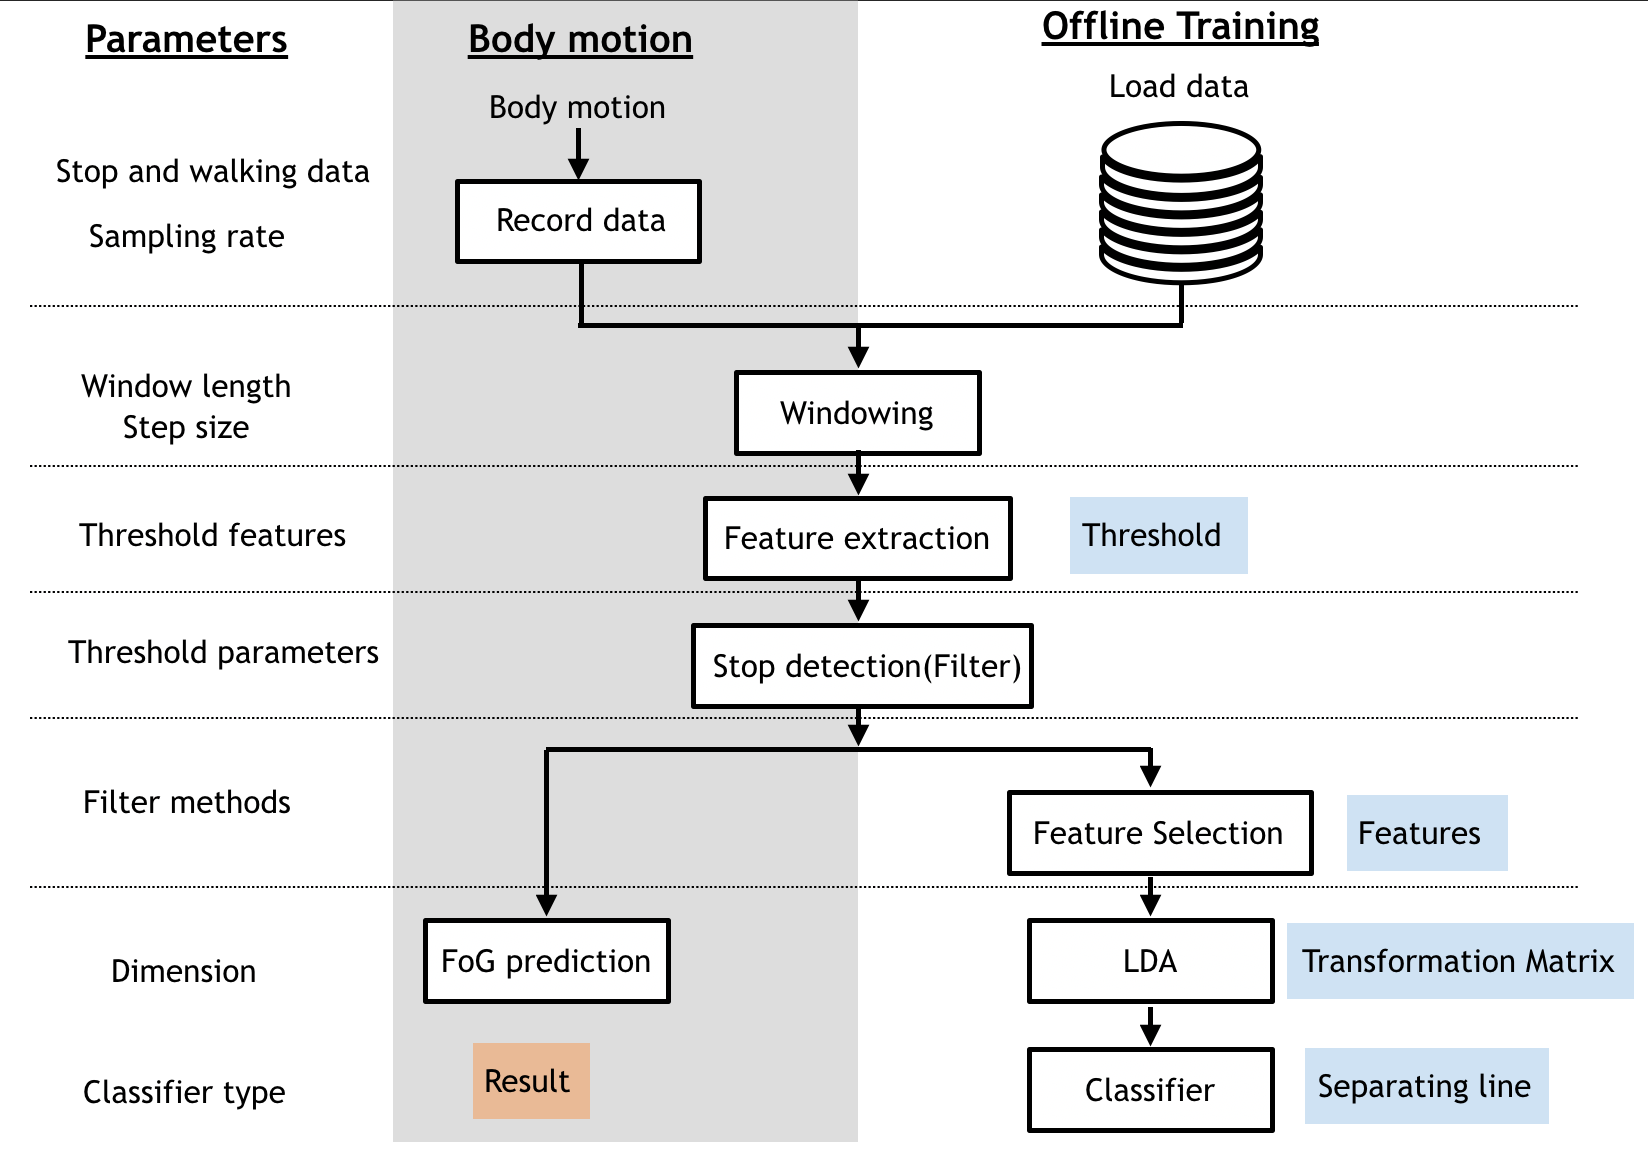
\includegraphics[width=0.47\textwidth]{procedures}
    	\caption{Working flow}
    	 \label{fig:procedure}
    	
    \end{figure}


% Method
\section{Method}

As mentioned before, some methods focusing on finding a good feature and used thresholds to detect FoG episodes \cite{FI}\cite{FI1}\cite{WM} , while the others applied machine learning methods to extract features and do classification \cite{Flo}\cite{ML}.

In the proposed method, we combine these two method together.

According to previous experience, it is hard to use LDA or PCA directly on raw data or low-pass filtered data to extract features with generality because of the unbalanced dataset and noises within.
However, the result with test set improves a little when LDA is performed with extracted features. 

The workflow of method is as figure \ref{fig:procedure} illustrates.
 after a window pre-processing step, several features are extracted from it.
\begin{enumerate}
\item Windowing approach to segment raw acceleration data into windows of equal length
\item For each window, several features are extracted
\item Thresholds are applied to clean dataset
\item Using mutual information and spearman's rank correlation to do feature selection		
\item Using LDA for feature extraction
\item Using Decision tree for classification with new quality metrics
 		
\end{enumerate}

More detail in going to be introduced in the following subsections.


\subsection{Windowing}
    \begin{figure}
	\centering
	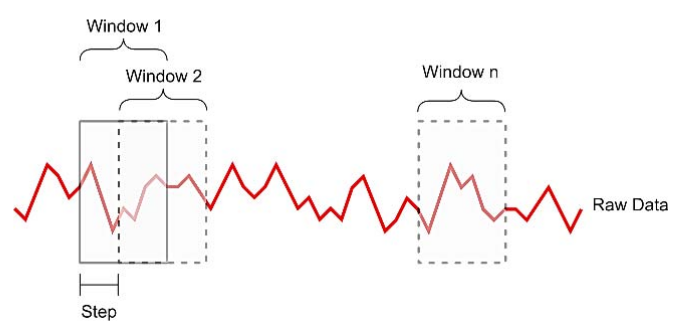
\includegraphics[width=0.47\textwidth]{windowing}
	\caption{Windowing approach to segment raw data into windows }
	\label{fig:windowing}
	
	\end{figure}
In order to extract features from raw acceleration data, we used sliding rectangular window function to get segments from dataset as figure \ref{fig:windowing} shows. The length of window and step length are variables in several researches \cite{Flo}\cite{ML}, it is possible to do a grid search for a best fit. There exists a trade off between window size and reaction time. We do not put too much effort in these parameters and set them as fixed which performs well for several other methods.

The size of sliding window is chosen as 2 seconds. The sampling frequency of dataset is 64 Hz, so each sensor contains 128 integer data in each axis, in total we have 128*9 integer data in the window. The step length is the shift between two windows, we set it as 0.5 seconds in out case. They are going to be the basis for feature extraction in next step.  

% Features Extraction

\subsection{Feature Extraction}

There are lots of researches focus on features of FoG episodes and some of them are used in the method \cite{FI}\cite{FI1}\cite{WM}\cite{sammpleE}, here I also used one feature found by muself.

the feature extraction can be performed in both time domain and frequency domain. 

\begin{figure}
\centering
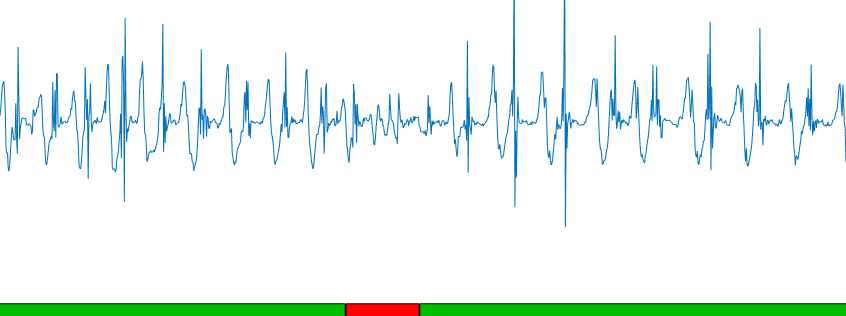
\includegraphics[width=0.47\textwidth]{periodic}
\caption{The green area(non-FoG) area has more periodicity than read area(FoG) in time domain}
\label{fig:periodic}
\end{figure}	
From the observation of acceleration data in time domain\ref{fig:periodic}, we can visualize clear some periodic pattern during the normal walking phase, However, such characteristic is less obvious or not existing in FoG phase. Since the window length is chosen as 2 seconds in our setup, generally at least two steps can be observed for most patient. The following three methods can be applied to exploit this periodicity.

	\begin{enumerate}
		\item Sample Entropy: A measure of complexity, Often used to analyze the physiological variability in human gait and it is derived from approaches developed by Richman and Moorman\cite{sammpleE}. A feature which shows the repeatability and predictability within one window. Suppose in one axis of one sensor, we have time-series of data of length N with constant time interval $\mathbf{X={[x_1,x_2,...x_N]}}$. Then we define another array with size m $\mathbf{X_m(i)={[x_i,x_{i+1},...x_{i+m-1}]}}$ and distance function $\mathbf{d =[ X_m(i)-X_m(j)]}$, the sample entropy is defined as:
    
		    \begin{equation}
		        \mathbf{SampEn(m,r,N)} = -log(\frac{A^m(r)}{B^m(r)})
		    \end{equation}
   
   		where A is equal to the number of template vector pairing  having $\mathbf{d[ X_{m+1}(i)-X_{m+1}(j)]<r}$

		B is equal to the number of template vector pairing  having $\mathbf{d[ X_{m}(i)-X_{m}(j)]<r}$
		
		   		
		In this study the dimension m is selected as 2, r as 0.2*$\mathbf{\delta}$, where $\mathbf{\delta}$ is standard deviation as previous papar did\cite{sammpleE}. 
  
		
	\item Cross Correlation : Another method to exploit the periodicity is to use cross correlation. This shows the similarity between a signal and its shifted version. The window size in our case is selected as 2 seconds, so generally 2 to 3 steps can be observed in it. In this way,a shift with highest value can be considered as a step interval. The window length is n, f(n) is the raw data set.
		
		\begin{equation}
		\mathbf{CrossCorrelation} = \sum_{n=0}^{n=len} f[n]f[n+\delta]
		\end{equation}
		
		Besides, the highest correlation value also shows the possibility of existing a periodic pattern in this window, which can be used as another feature.

	\item Fast step detection: Both methods mentioned before is quite expensive in terms of time, and when it is implemented on hardware the realtime capability might not be guaranteed. 
		
		Therefore, we invented a more light weight method based on the observation from data. As figure \ref{step} shows, A step usually comes with a large drop and rise in the acceleration data, such U shape can be used as a feature to detect one step. As the figure shows, we can search for continuous decrease in the value and find potential step points. With such information we can find the step interval, step frequency. The threshold to get classified as a U shape is different individually and need to be calculated using normal walking gait data, such as the blue part in figure \ref{ori}.
		
		The result is as the figure \ref{interval} shows, between 50 and 250 we can clearly see the patient is walking normally, so the step interval most of time stays at 60ms. Whenever the patient turns, we can clearly observe some gap. When the patient experience FoG, the step interval can decrease to 0 for patient 2.	

	\end{enumerate}

\begin{figure*}
	
	
	\begin{subfigure}[b]{0.47\textwidth}
		\centering
		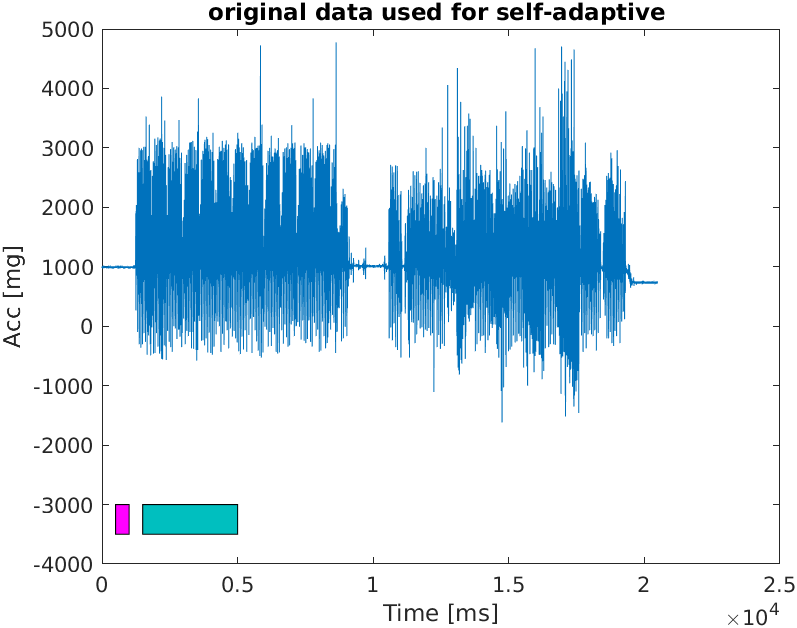
\includegraphics[width=\textwidth]{training_data_s2_p2}
		\caption{acceleration in x axis of ankle sensor}
		\label{ori}
	\end{subfigure}
	\hfill
	\begin{subfigure}[b]{0.47\textwidth}
		\centering
		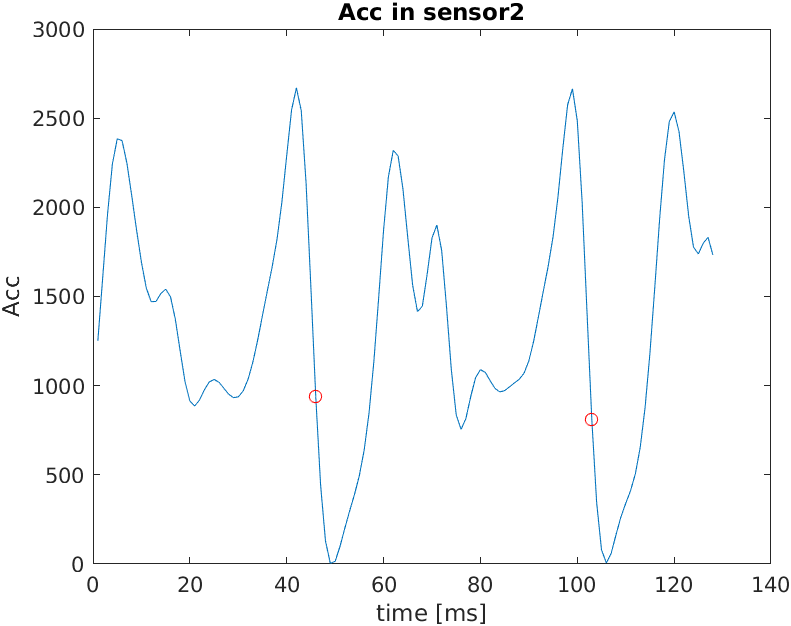
\includegraphics[width=\textwidth]{acc_step_s1_p2}
		\caption{acceleration of walking in y axis of ankle sensor}
		\label{step}
	\end{subfigure}
	\hfill
	
	
	\begin{subfigure}[b]{1\textwidth}
		\centering
		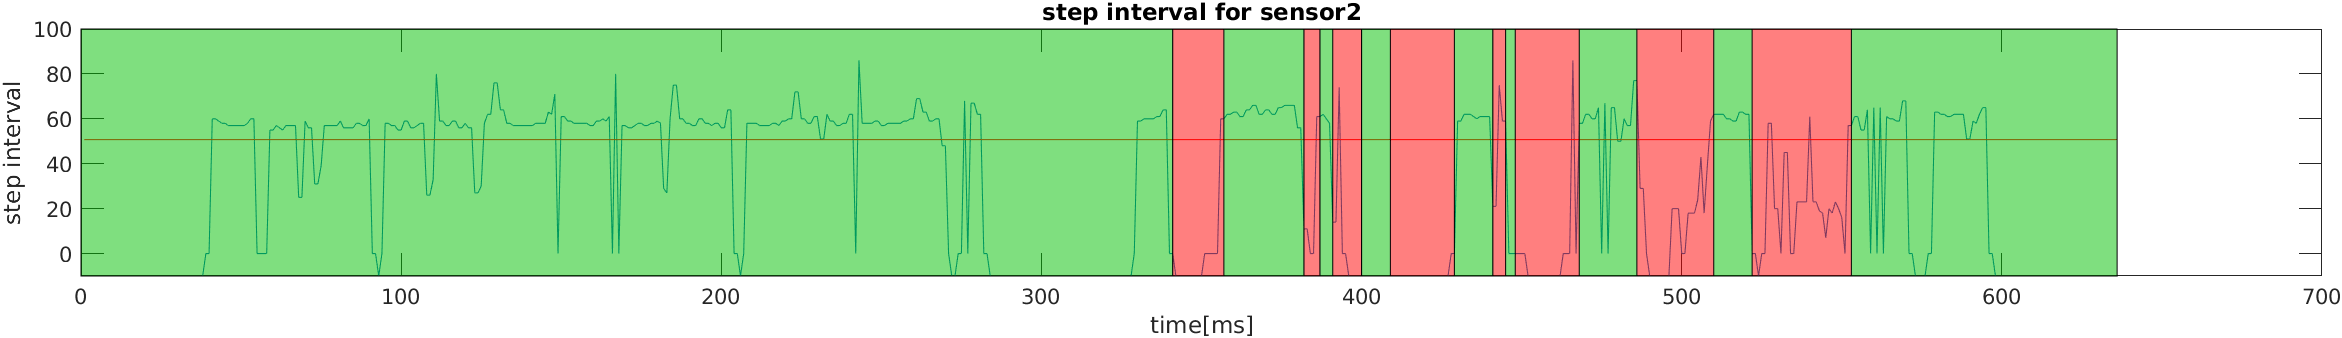
\includegraphics[width=\textwidth]{step_interval_fast_s2_p2}
		\caption{measured step interval}
		\label{interval}
	\end{subfigure}
	
	
	
	\caption{The red area shows FoG, the green area shows non-FoG(a)The acceleration in y axis of ankle sensor, the purple part shows stop, the blue part shows normal walking.(b)Zoom into one of the walking window, two U shape can be observed, the red point shows the detected step.(c)The time interval between two detected points shows where the FoG might be}
	\label{fig:three graphs}
\end{figure*}

	From another point of view, we can also extract useful information from frequency domain.

	\begin{enumerate}
		\item Dominant frequency peak: Dominant frequency is defined as the highest magnitude frequency in a power spectral density. This is the frequency which carries the most energy. Generally speaking, this value should coincide with step speed of walking during normal walking, which is 1-2 Hz. 
	
		\item Freezing Index and energy thresholds: Moore et al. discovers that more energy components appears
			in [3-8Hz] band during FoG \cite{FI}. They introduced a freeze Index(FI) as a strong indicator of FoG.
			
			To calculate FI, we apply a method proposed by Baechelin et al., they used a fast Fourier transform(FFT) to get power spectral density \cite{FI1}. The locomotion energy is calculated as the integral in [0-3Hz], and freeze energy is integrated in [3-8Hz]. The freeze Index is calculated as :
			\begin{equation}
			\mathbf{FI} = \frac{freezeband\,energy}{locoband\,energy}
			\end{equation}			


	
		\item Wavelet mean: Wavelet transform is a standard tool that shows how the power amplitude of a specific frequency in a signal change over time. In the paper of Rezvanian and Lockhart et al. \cite{WM}, they used the ratio of sum of wavelet coefficient in freeze and locomotion bands to discriminate FoG and non-FoG events. Here we used the mean of absolutes values of Discrete Wavelet Transform(DWT) from level three which includes freeze band. 
	
	\end{enumerate}

 Besides, some other features are included in the analysis, a summary is found in table 1.
\begin{center}
	\begin{table}
	\begin{tabular}{ |p{2cm}||p{6cm}|  }
		\hline
		\multicolumn{2}{|c|}{Features in time domain} \\
		\hline
		Features & Description\\
		\hline
		sample entropy & Measures repeatability or predictability within one window : \\
		\hline
		step interval & Time interval between two steps in one window\\
		\hline
		max correlation & Measures the periodicity in one window\\
		\hline
		step depth & Difference between max and min value in one window\\
		\hline
		step counts & Counts of steps in one window \\
		\hline
		variogram & The measure of smoothness of data in time series \\
		\hline
		portion above mean &The proportion above the mean of the observationswithin the window whose values are greater than
		the mean of the window \\
		
		\hline
		\multicolumn{2}{|c|}{Features in frequency domain}
		\\
		\hline
		Features & Description\\
		\hline
		loco-band energy & energy in [0.5-3Hz] frequency band\\
		\hline
		loco-band+freeze-band energy & energy in [0-8Hz] frequency band \\
		\hline
		freezing index & The power in the 3-8Hz band divided by the power in 0.5–3 Hz band  \\
		\hline
		dominant frequency & The frequency with maximal Power Spectral Density (PSD) \\
		\hline
		wavelet mean & the mean of coefficient of DWT in the third level, which represents energy in freeze band \\
		
		\hline
	\end{tabular}
\label{ft1}
\caption{Features extracted from windows}
\end{table}
\end{center}


	
\subsection{Thresholds and data cleaning}
This part is added into the process in order to clean the data and relabel some windows. As mentioned before, the original labeling performed by experts may have the problem of delay and not precise. Here I would like to give an example. 

The figure\ref{fig:thresholding1} shows original labels and acceleration data for patient 8, the red area below shows FoG labels and green area shows non-FoG labels. We can see something interesting happens in the beginning part of FoG data, however, we cannot see significant difference between the later 2/3 part of FoG and stop status of patient as the non-FoG part follows. This similarity may cause some confusion to feature selection, LDA and classification. 

Therefore, it is reasonable to clean this data before continue. In this method, we use thresholds for some features to do the cleaning. For example, in the case of patient 8, we can use sum of energy in freeze band and locomotion band to detect the stop-like period and delete them from training set. 

Another advantage of introducing thresholds is that we can filter some windows away that are alike to non-FoG based on previous knowledge and typical characteristic. It reduces the workload of procedures after it and helps them concentrate more on discriminating and classifying true FoG winodws and FoG-alike non-FoG windows. It also makes the training data less unbalanced.

It worth mentioning that some other features and thresholds can be applied for the same purpose. For example, as figure\ref{fig:thresholding2} illustrates, the non-FOG part shows obvious more periodic pattern in compare with FoG area, we can also use it as a thresholds to filter away periodic parts. 

To make sure the final result is comparable with other methods available, we must make sure all non-FoG windows and FoG windows filtered away by the threshold method are present in the final validation step. We use the following setup as figure\ref{fig:validation} shows to prepare training data and validation data. After the classification is finished, the result is filled with windows that were filtered, they are labeled as non-FoG, the validation is performed between original label and extended result.

\begin{figure}
	\begin{subfigure}[b]{0.43\textwidth}
	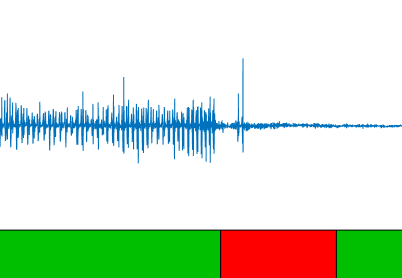
\includegraphics[width=\textwidth]{patient8_ori_lda_label}
	\caption{raw acceleration data of patient 8 with labels}
	\label{fig:thresholding1}
	\end{subfigure}

	\begin{subfigure}[b]{0.43\textwidth}
		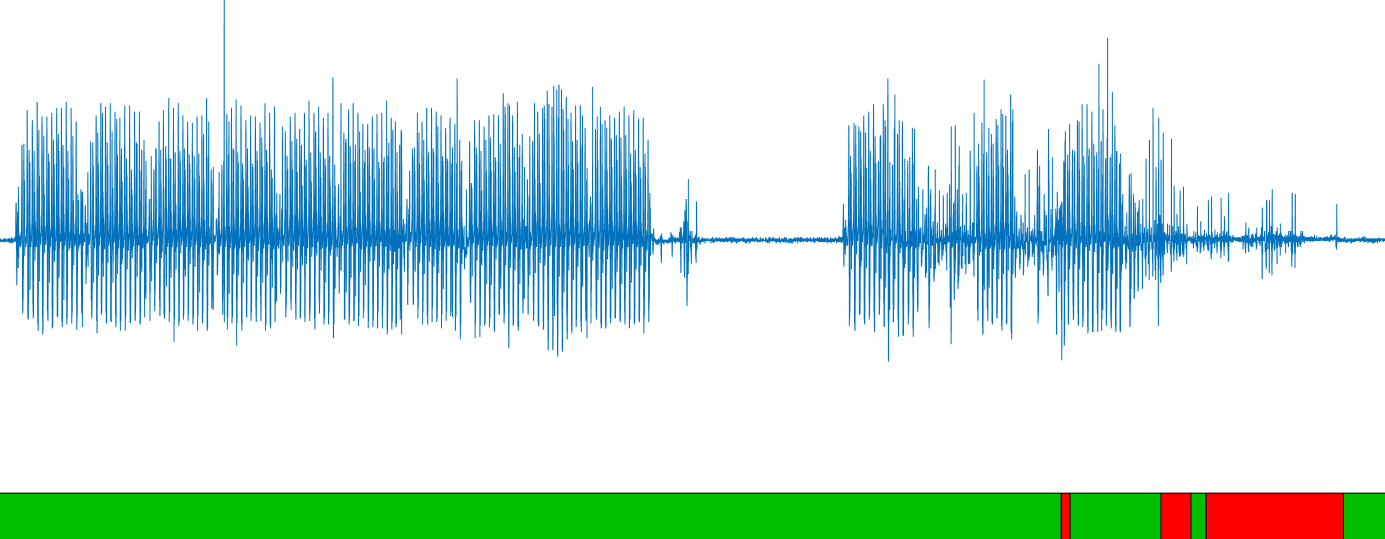
\includegraphics[width=\textwidth]{p6_lda_ori}
		\caption{raw acceleration data of patient 6 with labels}
		\label{fig:thresholding2}
	\end{subfigure}
	\caption{raw acceleration data of patient with labels}
\end{figure}

\begin{center}
	\begin{figure}
		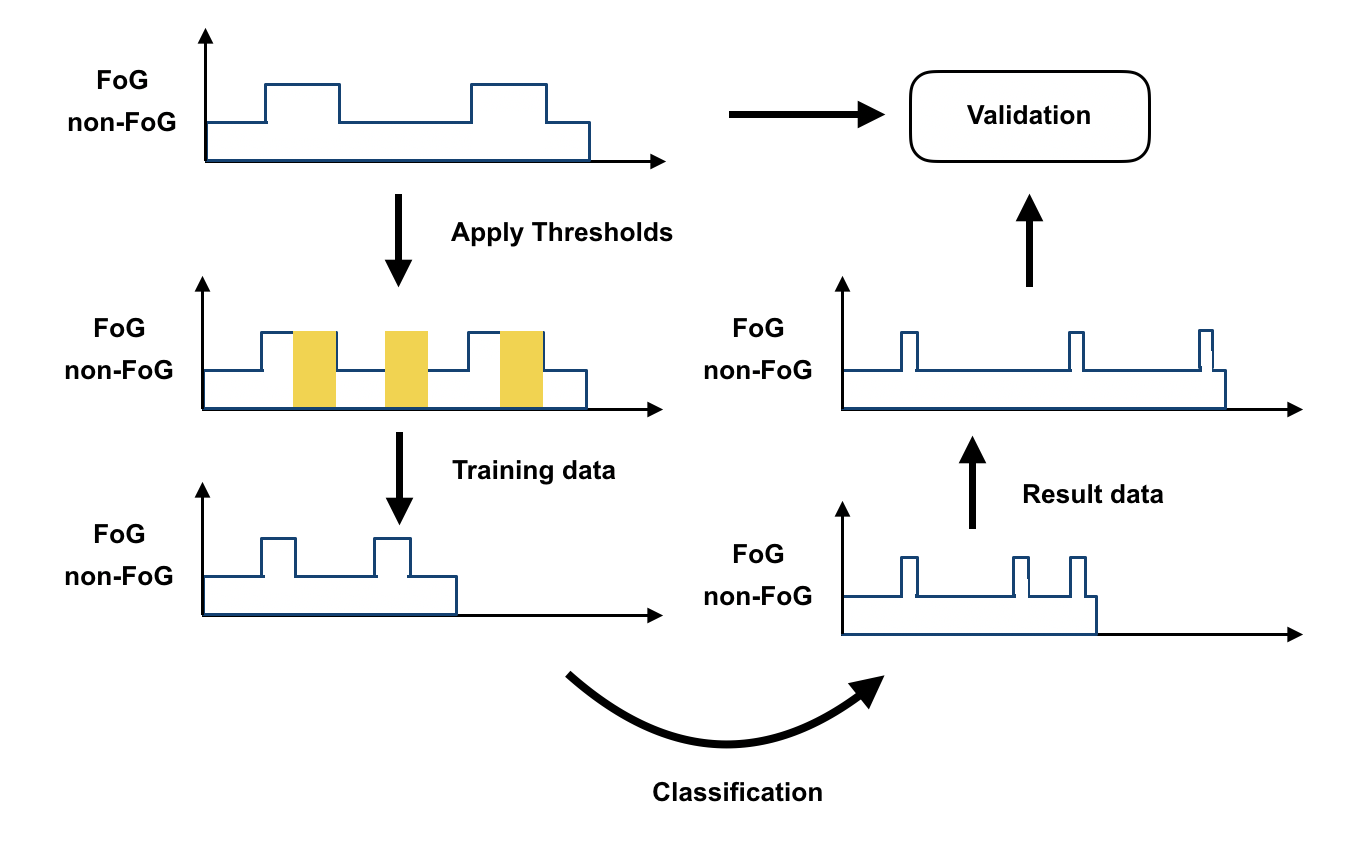
\includegraphics[width=0.5\textwidth]{VALIDATION}
		\caption{Validation under the threshold method}
		\label{fig:validation}
\end{figure}
\end{center}


\subsection{Feature Selection}

After the features are extracted, and non-FoG alike windows are filtered away. Generally we can just feed them into a dimension reduction tool like LDA. However, the result of using features directly does not generate good results.

According to the observation, different features have different dependencies with labeling. Also, different patients have different gait features during the FoG, therefore, it is important to find out which features are more efficient for each patient. This can be explained with the fact that different patients have different symptoms during the FoG, according to the research of Parisa Tahafchi et al.\cite{symptoms} FoG can be shown as festination, akinesia and trembling, and such different symptoms have different dependencies with features. 

Although LDA is capable of selecting not meaningful features out by giving them very small weights, but this ability is fully depend on the quality of data set.

We selected filter method to do feature selection, because it selects features independently from any classification algorithm. It helps us remove features that contain little information .

Correlation filter method such as Spearman's rank correlation can be used to measure the degree of association between two set of variables with a monotonic function. It is capable of handling non-linear functions in compare with Pearson correlation.

Statistical method such as mutual information a measure of the mutual dependence of two variables. It measures the amount of information obtained about one variable through observing the other variable. 

In the experiment we are going to use both of them and make comparison.


\subsection{Feature reduction}

After we get the cleaned dataset and selected features, we are ready for LDA. Since simple thresholds on all these features is still too complicate and computational expensive. We still need this step to further reduce the dimension down to a level which is easier for classification.

The output dimension of LDA is depends on classification method. Higher dimension comes with higher performance at the cost of more computation and memory resource requirement.

The simplest version of classifier is dealing with one dimensional features. In such case, the classifier only need to draw a line and discriminate the data based on this threshold, as in figure \ref{lda1}. The last step is to design a classifier which gives us this line. It is worth noted that the design of classifier is closely coupled with evaluation standard, which need to be clarified first.


% Evaluation standard

\subsection{Classification and Evaluation standard}



	All papers regarding the FoG detection uses classical classification quality metrics,such as precision, specificity Recall and F1-Score.
	
	However, such classification standard does not consider the user experience and application characteristic. From our observation, there are some phases during FoG where the features can be different. Some part of FoG episodes are more different from normal gait than the others. For example ,the beginning of a FoG phase is more likely to get classified as a FoG window in compare with others and some part inside a FoG episodes do not differ much from a normal stop or normal walk. As figure \ref{lda1} shows, the last part of first and second FoG  mixed together with normal gaits. 
	
	Another observation is with the third FoG episodes, some windows before the FoG windows are also classified as FoG window. This may be due to that there is a delay before the start of disease and observation or it is invisible. However, such miss classification actually helps us to detect the FoG before it actually happens.

	In summary, a traditional way of evaluation may not be the best option in this case, it is reasonable to make some changes for a better performance and result.
	
	From one side, since the objective is to detect FoG in a realtime way, it is desired that the time window before the actual FoG is also classified as a FoG.
	
	From the other side, the detector may label several windows that are found inside a FoG labeled sequence as non-FoG, however, such false detected points does not have a high cost in real life, since the patient can recover from the FoG as long as he get an alarm for a certain time in the beginning part. It is more important not to make false alarm when the patient is walking normally. 
	
    Besides, considering that a false alarm happens just after the FoG is not so annoying as a false alarm during a normal walk, we also consider it as a correct label.
    
    In conclusion, the following situations need to be reconsidered, as shown in figure \ref{eva}:

    \begin{enumerate}
    	\item The FoG rising edge: If one continuous window sequence before the rising edge is classified as a FoG period, then the whole window sequence is considered as correct labeled even part of them are not labeled as FoG in the dataset. In figure \ref{eva}, the first Detected FoG Signal is one of such case, and it is a correct detection.
    	
		\item During the FoG period: If the edge is detected and solved with one filter window, the whole continuous FoG period is considered as solved.  In figure \ref{eva} the first FoG window is considered as solved, even the Detected FoG Signal does not cover all of it. Otherwise, if the FoG is detected after the coming edge, only part of the FoG period is considered as solved, like in the second Labeled FoG Signal situation, only part of it happens after a detection.
		
		\item Whenever one FoG period ends, if one continuous window sequence is correct labeled at this point, then all filter window continuously followed are considered as correct.		
    \end{enumerate}

	In this way, such evaluation standard does not punishes the wrong results that 
	after a correct FoG beginning detection and reward the part the detection before beginning of FoG. We make the detector focus more on the beginning part of FoG phase instead of whole part, It also makes less annoying false alarm.
	In this way, we have a new evaluation standard. New Precision stands for the percentage of correct alarm in all windows labeled as FoG, which is similar to Precision. New Recall stands for how many FoG windows are solved, which is the similar as recall before.
	
	\begin{equation}
	\mathbf{New\,Precision} = \frac{\sum corrcect\,FoG\,alarms}{\sum all\,FoG\,alrams}
	\end{equation}
	
	\begin{equation}
	\mathbf{New\,Recall} = \frac{\sum solved\,FoG}{\sum all\,FoGs\,exists}
	\end{equation}
	
	\begin{equation}
	\mathbf{New\,F1-Score} = 2*\frac{New\,Precision * New\,Recall}{New\,Precision+New\,Recall}
	\end{equation}
	
	
	To find a separating line, we apply the same method as in decision tree. Several possible thresholds between the mean of FoG features and non-FoG features is selected, then the quality metrics is calculated to find out the best threshold. 
	
	\begin{figure}	
		 \begin{center}	
	\begin{subfigure}[b]{0.45\textwidth}
		\centering
		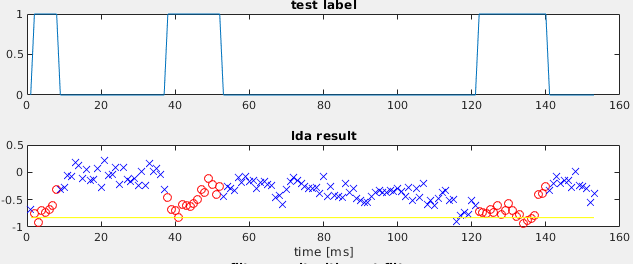
\includegraphics[width=\textwidth]{p8_lda}
		\caption{lda result and test label}
		\label{lda1}
	\end{subfigure}

	\begin{subfigure}[b]{0.45\textwidth}
	\centering
	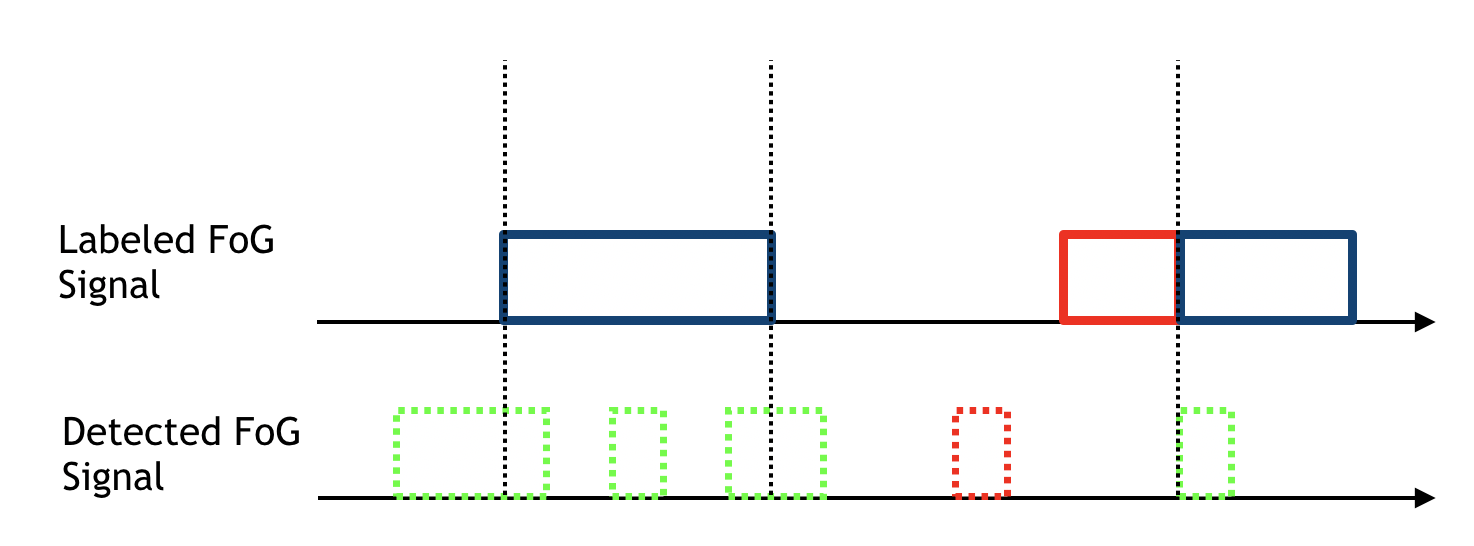
\includegraphics[width=\textwidth]{evaluation}
	\caption{Evaluation method}
	\label{eva}	
	\end{subfigure}
	\caption{(a)The blue line shows the mean value of features in non-FoG windows, the red line shows the mean value of features in FoG windows. The target is to find a separating line(yellow) which best discriminate the data}

\end{center}
\end{figure}
	In decision tree algorithm, generally gini index is going to be used, However, it does not performs so well with unbalanced data since the line is always too agressive with high recall and low precision. So we tried to use a  scaled version of gini index in which we make each FoG points n times bigger in terms of number, n is the ratio of number between the non-FoG points and FoG points. Also we can use the new evaluation standard and try to find a best result with highest F1-score.
	

	
% Classifier design
\section{Result}
 \begin{table*}
	\begin{center}
		\begin{tabular}{  |p{0.5cm}||p{1.3cm}|p{1.3cm}|p{1.3cm}|p{1.3cm}|p{1.3cm}|p{1.3cm}|p{1.3cm}|p{1.3cm}|p{1.3cm}| }
			\hline
			\multicolumn{4}{|c|}{Result without thresholds} &\multicolumn{3}{|c|}{Energy threshold}&\multicolumn{3}{|c|}{Energy+Dominant frequency threshold}  \\
			\hline
			ID &  precision &  recall &  F1-score &  precision &  recall &  F1-score &  precision &  recall &  F1-score\\
			\hline
			1 & 0.7358 &0.8390 & 0.7840 & 0.7222 &0.8764 & 0.7919 & 0.6905 &0.8764 & 0.7724\\
			2 &0.6588 & 0.7982  & 0.8277 &0.8009 & 0.9286 & 0.8141 &  0.8552 &0.8555 & 0.8553\\ 
			
			3 & 0.7545 &0.8873 & 0.8155 & 0.7541 &0.8802 & 0.8123 &  0.7859 &0.8730 & 0.8272 \\   
			
			5   & 0.7288 &0.8986 & 0.8048  & 0.7903 &0.8923 & 0.8382 & 0.7753 &0.9333 & 0.8470\\
			
			6  & 0.4685 &0.8581 & \cellcolor{blue!25} 0.6061 & 0.5415 &0.6990 & 0.6102 & 0.6713 &0.8651 & \cellcolor{blue!25} 0.7560\\
			
			7& 0.6084 &0.8130 & 0.6960&  0.6667 &0.7609 & 0.7107  & 0.6787 &0.7957 & 0.7325 \\
			
			8  & 0.7380 &0.8288 & \cellcolor{blue!25} 0.7808 & 0.8317 &0.8927 & \cellcolor{blue!25} 0.8611 & 0.8170 &0.9292 & 0.8695  \\	
			
			9  & 0.7896 &0.7071 & \cellcolor{blue!25} 0.7460 & 0.8439 &0.9135 & \cellcolor{blue!25} 0.8774 & 0.8534 &0.9250 & 0.8877\\
			\hline
		\end{tabular}
		\caption{Comparison with feature threshold as an additional step}
		\label{thresholds}
	\end{center}
\end{table*}
	The validation is conducted using 10-fold cross validation with all patient except patient 4 and patient 10, each training process is conducted with individual data separately. 

	Table \ref{thresholds} shows the effect of applying thresholds. We first used total energy in locomotion and freeze band as an indicator of stop status, it helps patient 8 and patient 9 improve its F1-score for 8\% and 13\% separately. Adding dominant frequency as another threshold, the F1-score of patient 6 improves by 15\% while it does not effect others too much if not helps. This proves our assumption that data cleaning can help improve the performance of classifier.
    
	The second result worth mentioned is feature selection. Using statistical tools we can figure out which features on which channel is really closely correlated with FoG symptoms.
    We calculate mean value Spearman rank correlation and mutual information of each feature value and labels for all patients, the result is shown in the Figure \ref{fs}. 
    
    When it comes to different patient, the efficient features will also be different. Generally speaking for all patient, the result of two methods coincide with each other. The three sensors placed in different locations and three axes can been seen as nine channels. From picture a and b, it is clear that channel1 (Horizontal forward acceleration on ankle), channel 2 (Vertical acceleration on ankle) and channel 5 (Vertical acceleration above knee) have the highest dependency with FoG symptoms. On the other hand, picture c and d shows the dominant frequency, locomotion energy and freezing index has the closest relationship with FoG among all features. According to the observation, since cross correlation, sample entropy and wavelet mean have quite low score and at the same time  they are quite expensive in terms of computation, we decide to throw them from the list of features.
    
    
   	\begin{figure*}
    	
    	\begin{subfigure}[b]{0.47\textwidth}
    		\centering
    		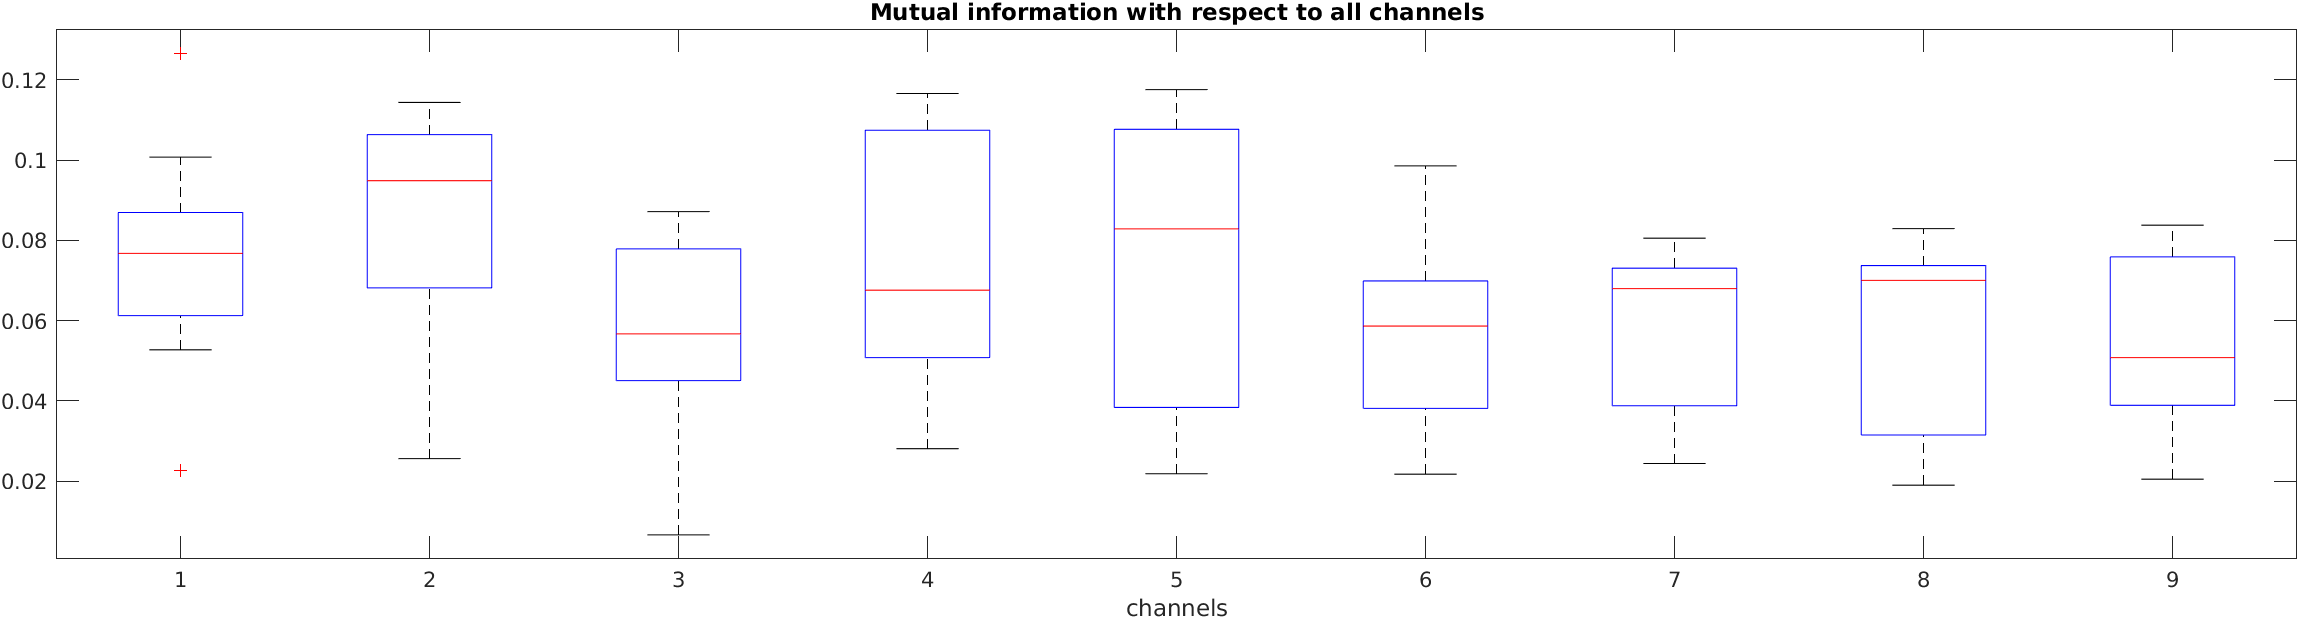
\includegraphics[width=\textwidth]{MutualA}
    		\caption{}
    		\label{fig:y equals x}
    	\end{subfigure}
		\hfill
    	\begin{subfigure}[b]{0.47\textwidth}
		\centering
		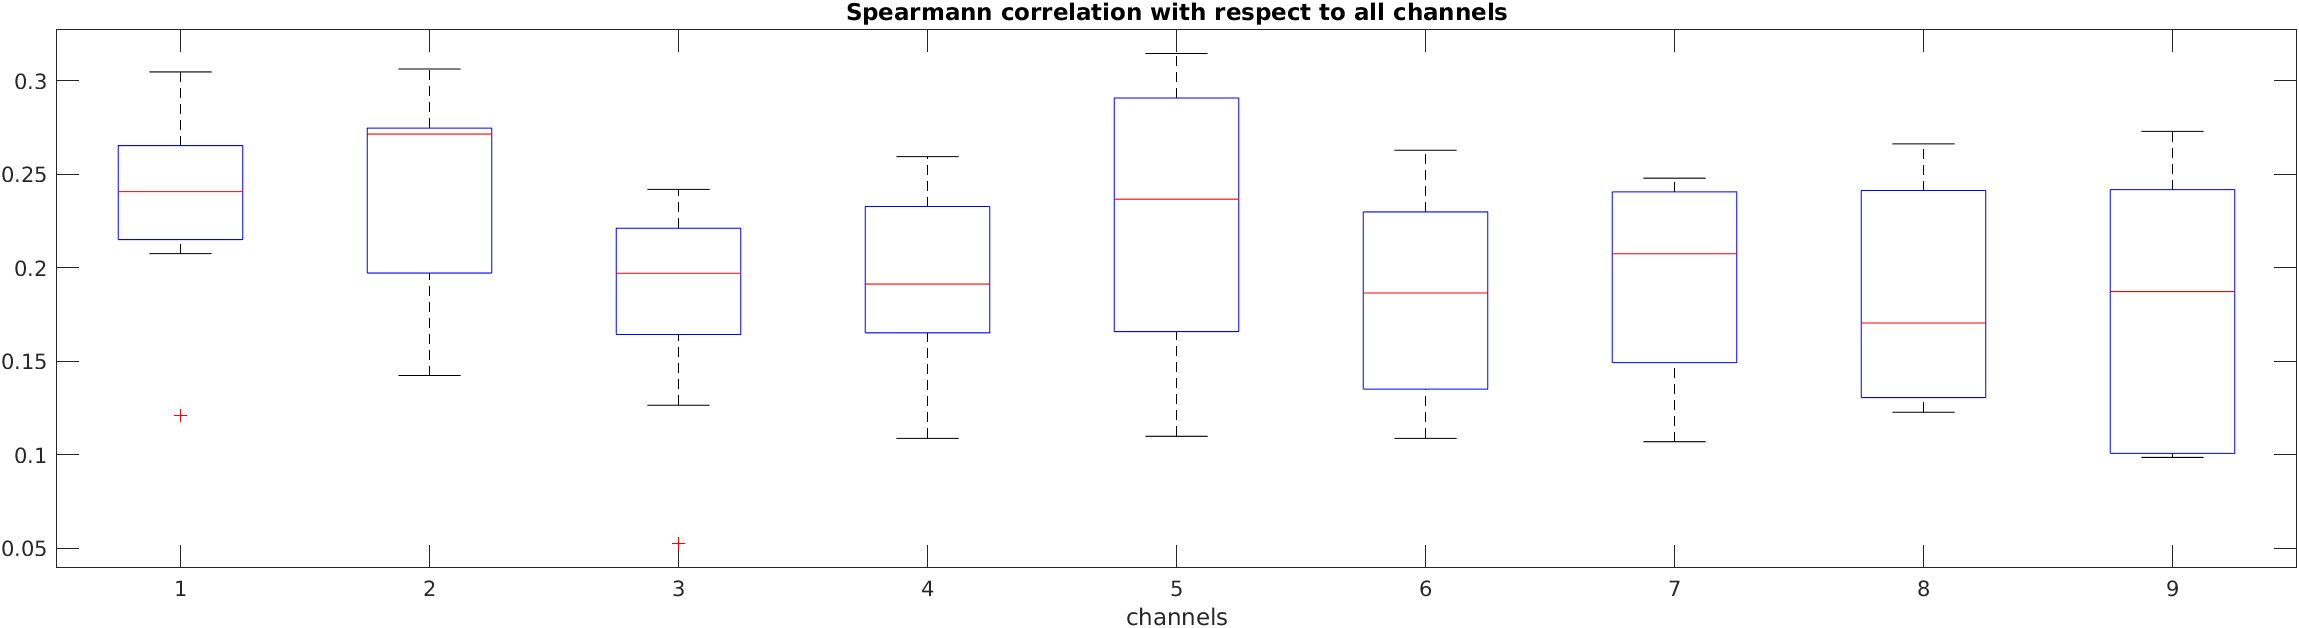
\includegraphics[width=\textwidth]{spearmannA}
		\caption{}
		\label{fig:y equals x}
		\end{subfigure}
	
		\begin{subfigure}[b]{0.47\textwidth}
			\centering
			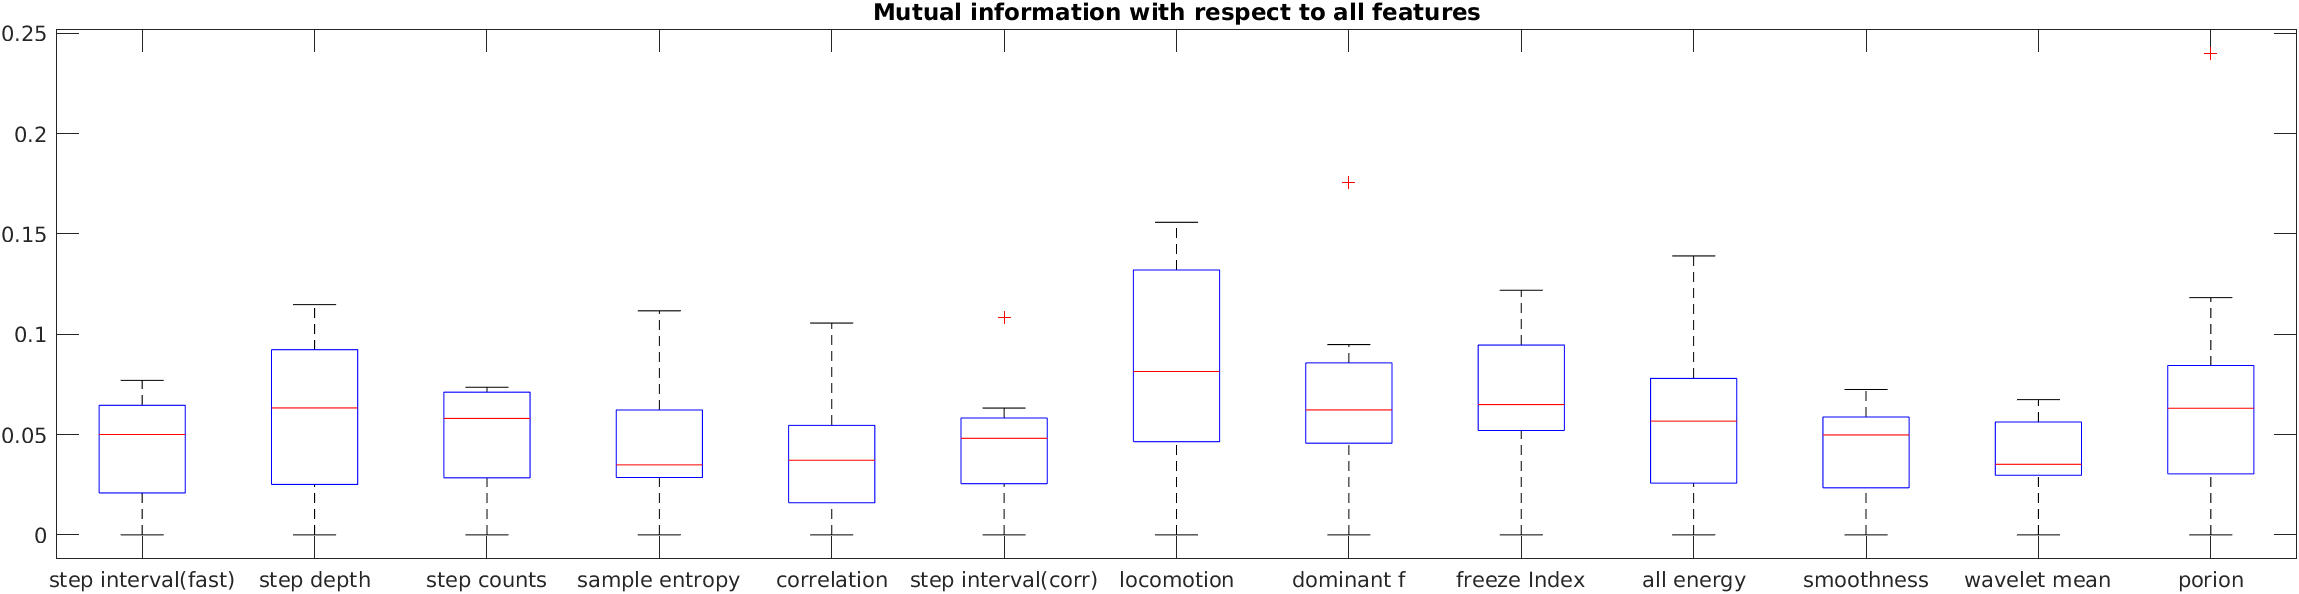
\includegraphics[width=\textwidth]{MutualF}
			\caption{}
			\label{fig:y equals x}
		\end{subfigure}
		\hfill
		\begin{subfigure}[b]{0.47\textwidth}
			\centering
			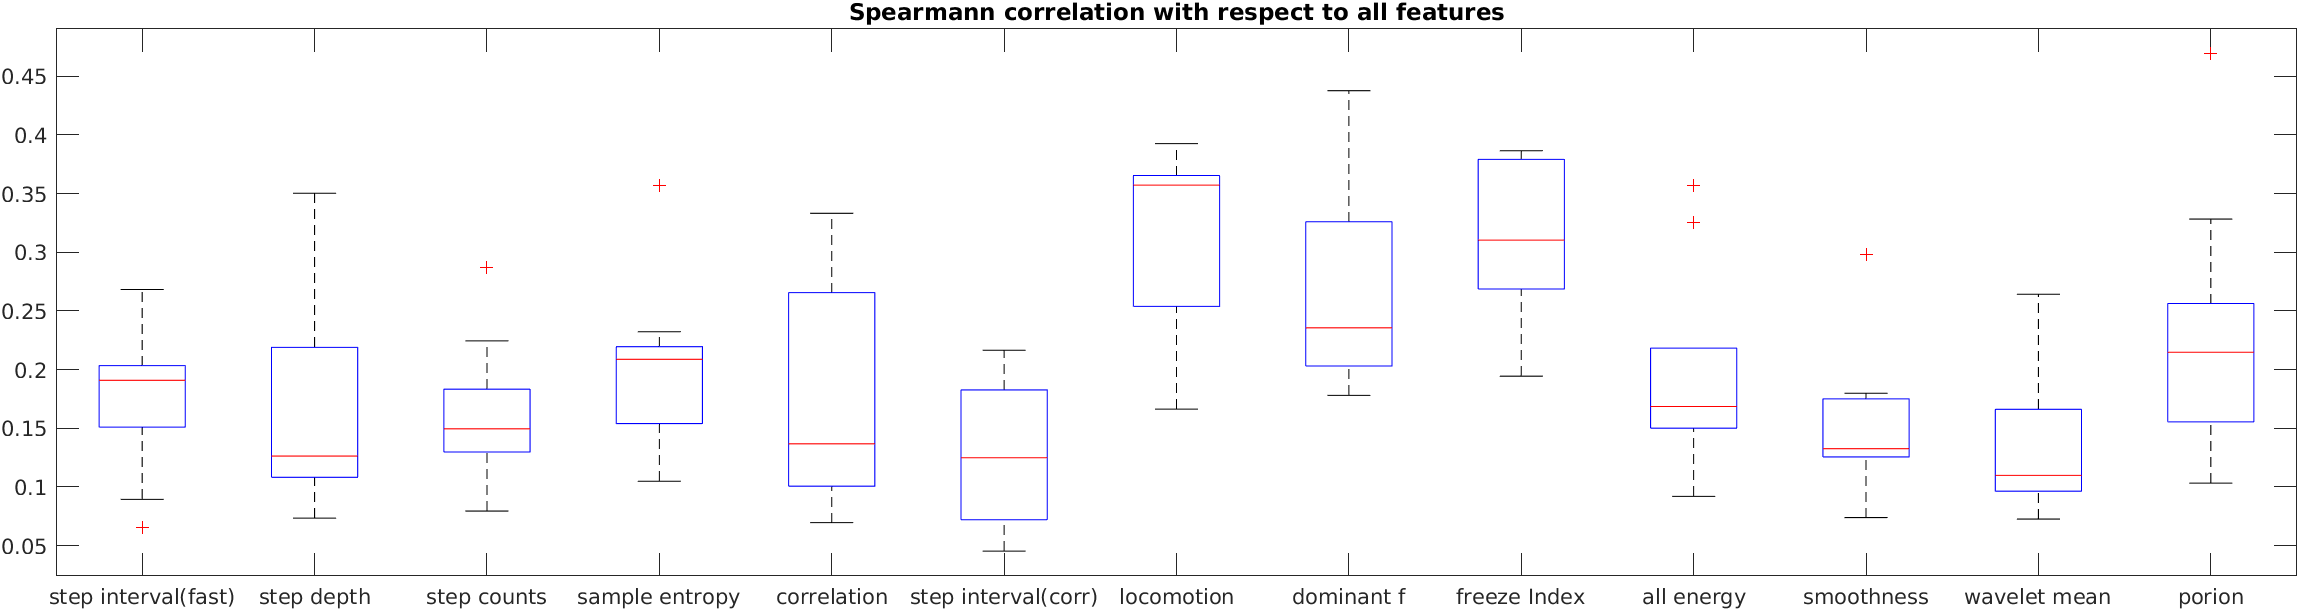
\includegraphics[width=\textwidth]{spearmannF}
			\caption{}
			\label{fig:y equals x}
		\end{subfigure}
    
    	\caption{Figure(a) shows the mutual information between channels and FoG;Figure(b) shows the Spearmann correlation between channels and FoG;
    	Figure(c) shows the mutual information between features and FoG;
		Figure(d) shows the Spearmann correlation between features and FoG;}
    	\label{fs}
    \end{figure*}
    
We use the threshold method to filter away features that have low score in terms of Spearman's rank correlation and mutual information separately and do classification. The classification result using new evaluation standard as quality metrics is shown in Table \ref{feature_s}.

 \begin{table*}
	\begin{center}
		\begin{tabular}{  |p{0.5cm}||p{1.3cm}|p{1.3cm}|p{1.3cm}|p{1.3cm}|p{1.3cm}|p{1.3cm}|p{1.3cm}|p{1.3cm}|p{1.3cm}| }
			\hline
			\multicolumn{4}{|c|}{Without feature selection} &\multicolumn{3}{|c|}{With Mutual information}&\multicolumn{3}{|c|}{With Spearman's rank correlation}  \\
			
			\hline
			ID &  precision &  recall &  F1-score &  precision &  recall &  F1-score &  precision &  recall &  F1-score\\
			\hline
			1 & 0.7222 &0.8764 & 0.7919 & 0.6905 &0.8764 & 0.7724 & 0.7000 &0.8090 & 0.7506 \\
			2 & 0.8333 &0.8412 & 0.8373  &  0.8552 &0.8555 & 0.8553 &  0.8469 &0.8768 & 0.8616\\ 
			
			3 & 0.7603 &0.8402 & 0.7983&  0.7859 &0.8730 & 0.8272 & 0.7988 &0.8588 & 0.8277 \\   
			
			5 & 0.8002 &0.9270 & 0.8589 & 0.7753 &0.9333 & 0.8470 & 0.7976 &0.9101 & 0.8502 \\
			
			6 & 0.5347 &0.8270 & 0.6495 & 0.6713 &0.8651 &  0.7560 & 0.6230 &0.8339 & 0.7132 \\
			
			7 & 0.6489 &0.7304 & 0.6873  & 0.6787 &0.7957 & 0.7325  &  0.7318 &0.8217 & 0.7742\\
			
			8 & 0.7928 &0.8105 & 0.8015  & 0.8170 &0.9292 & 0.8695   & 0.8080 &0.9178 & 0.8594   \\	
			
			9 & 0.8676 &0.9054 & 0.8861  & 0.8534 &0.9250 & 0.8877 & 0.8568 &0.9070 & 0.8812\\
			\hline
		\end{tabular}
		\caption{Comparison between different feature selection methods}
		\label{feature_s}
	\end{center}
\end{table*}




 \begin{table}
    \begin{center}
   		\begin{tabular}{  |p{0.5cm}||p{1.5cm}|p{1.5cm}| }
		\hline
		\multicolumn{1}{|c|}{Method}
		&\multicolumn{1}{|c|}{Proposed method}  &\multicolumn{1}{|c|}{Method\cite{FI1}}  \\
	
		\hline
		 ID &   F1-score  &  F1-score \\
		\hline
		1  & 0.7724 & 0.7056 \\
		2 & 0.8553   & 0.7658\\ 
		
		3 & 0.8272 & 0.8548 \\   
		
		5& 0.8470  & 0.8214 \\
		
		6 &  0.7560 & 0.6736 \\
		
		7  & 0.7325  & 0.6578\\
		
		8   & 0.8695  & 0.7951   \\	
		
		9  & 0.8877   & 0.7398\\
		\hline
		\end{tabular}
	\caption{detection result}
\end{center}
     \end{table}
   Then we can look closer to the result of detection in figure \ref{result}. The a figure shows the original method, and the b figure shows the result with new detector, it is clear than the number of false alarm decreases while most FoG windows are correctly detected. This makes sense, because under new evaluation standard, only false detection far away from real FoG period leads to a cost.
   
 
    
    \begin{figure}
    \begin{center}
    	
    	\begin{subfigure}[b]{0.45\textwidth}
    		\centering
    		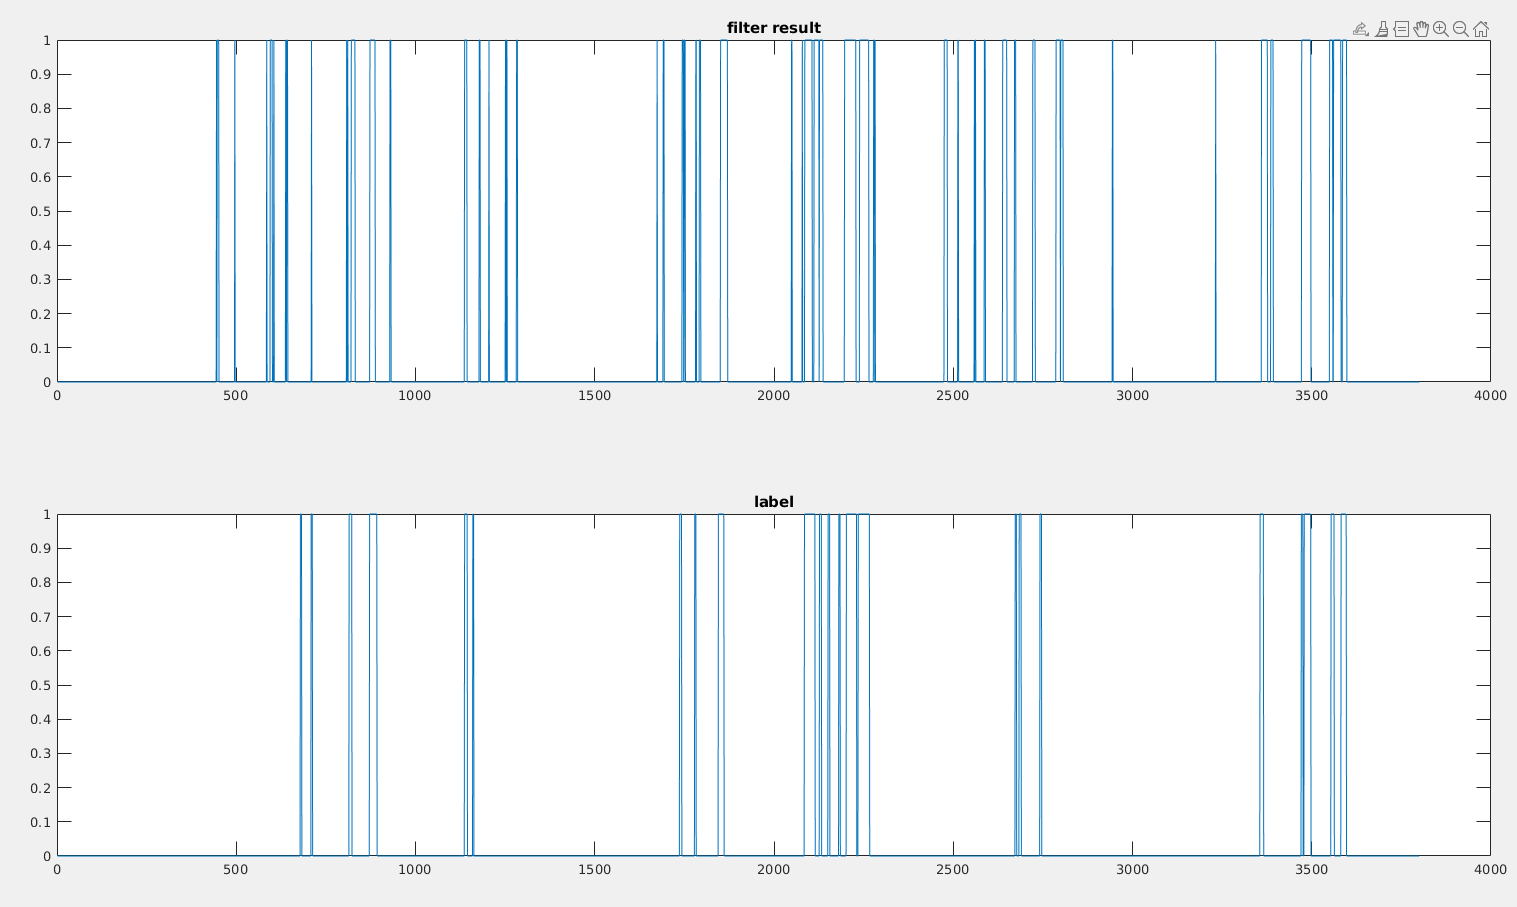
\includegraphics[width=\textwidth]{method1}
    		\caption{}
    	
    	\end{subfigure}
    	\hfill
    	\begin{subfigure}[b]{0.45\textwidth}
    		\centering
    		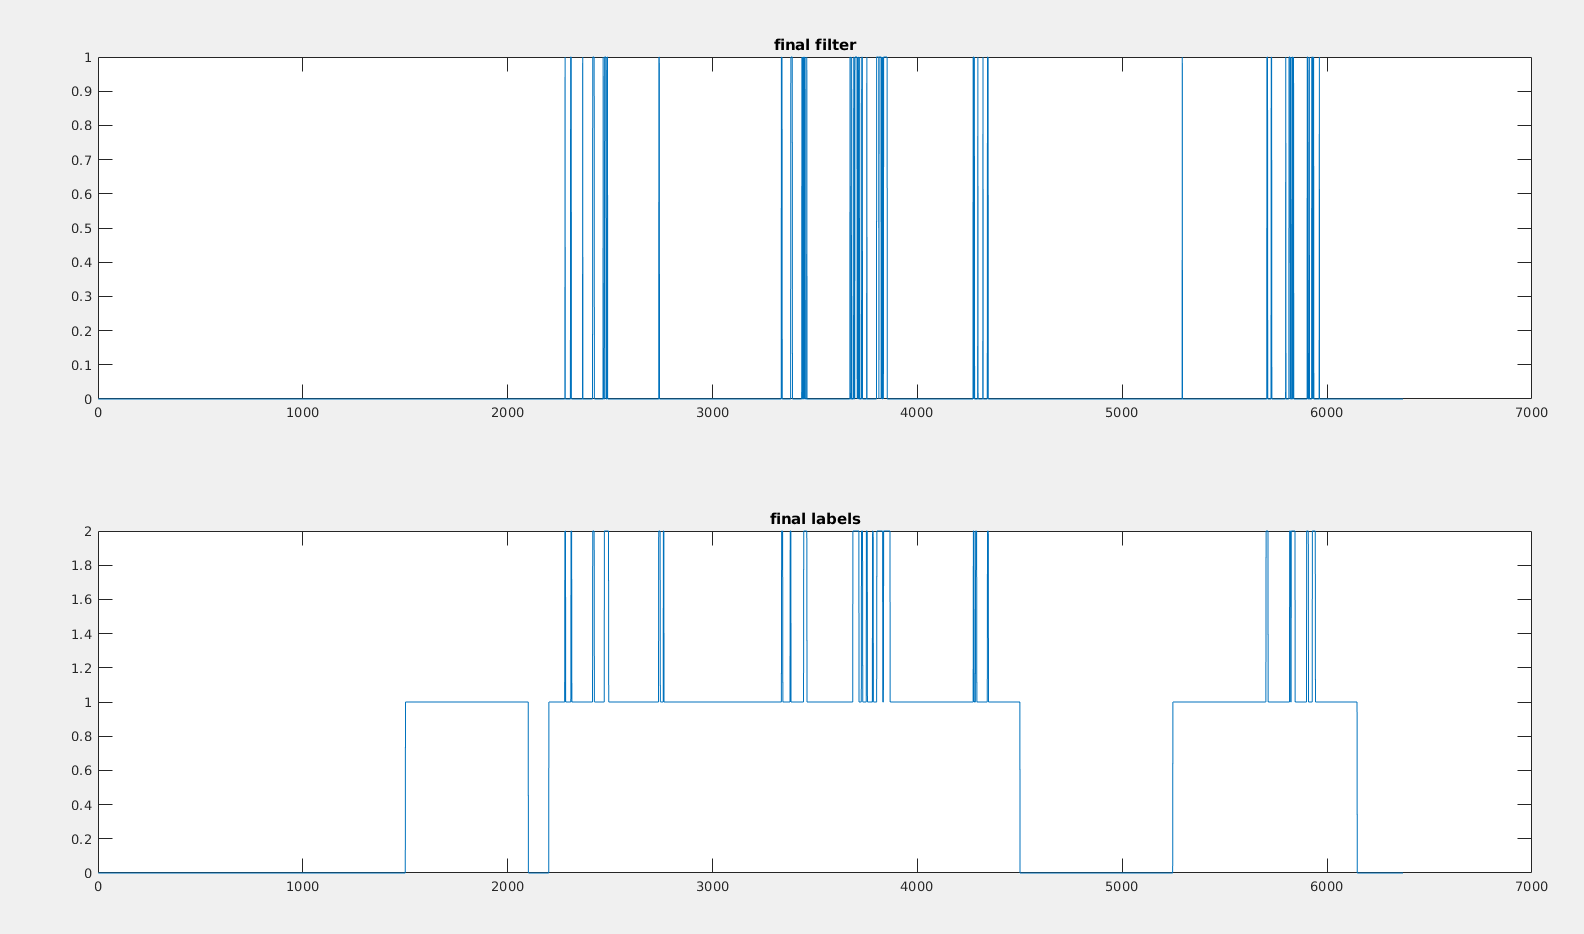
\includegraphics[width=\textwidth]{method2}
    		\caption{}
    		
    	\end{subfigure}
    	   	
    	\caption{Figure(a) shows the detection result use Bachelin's method and its comparison with label;Figure(b) shows the detection result use Spearman's rank correlation to select features and its comparison with label;}
    	\label{result}
 \end{center}	
   
 \end{figure}
    


% Hardware design
\section{Implementation}
   The implementation is mainly divided into three part: Graphic user interface implemented with Qt, data training written in python and C code that running on the hardware. Since we don't have sensors that does the measurement, UART is applied to send data in window form (128*9 integer) to the hardware. The hardware we used here is the nRF52 Development kit which has 512 kB flash and 64 kB RAM memory space.  
        
   
   In the graphic user interface, we can choose the auto mode which uses the method mentioned before to select features, or we can manually configure the sensors numbers and lda features. The manual configuration mode is available since expert can select features that meaningful for each person individually, it may outperform the auto method which is based on data. Besides, for both mode we can also select classifiers, thresholds and relevant parameters. 
   
   After the configuration part is done, relevant data will be feed into python code as parameters and training process starts. After the training process is finished, it returns and informs the user and save results into a file at the same time. 
   
   Then user can further use GUI to send results of training and raw data measurement in window form to hardware with UART, the hardware returns the detection result back to user interface before it receives new window.
   
	Code and more detail in found in git repository (https://github.com/wei2374/FoG\_detect).
   
  
% Conclusion and futhure work
\section{Conclusion and future work}
The focus of this research is to detect and predict FoG events in Parkinson Disease patients through feature extraction, feature selection and decision tree.
We invented a feature based on observation of raw data in time domain to exploit the periodicity characteristic of gait, it is computational less expensive in compare with other methods. A data cleaning idea is proposed and it helps the classifier make less false alarm. A new quality metrics is proposed, it focuses more on detecting the beginning part of FoG episode and has less tolerance to false alarms in compare with traditional metrics. In general, the result using new metrics shows great improvement in compare with original method proposed by the paper about DAPHNET dataset. In the future, more complicated classifiers can be employed to improve the performance.

As a direction for future investigation, other sensors can be applied to provide physiological information. It is also suggested to make modifications to feature selection algorithm, classification methods and classification quality metrics.  

    

\bibliographystyle{ieeetr}
\bibliography{other/bibliography}
\nocite{*}
		
\end{document}